% Chapter 9: Euler's Formula and Identity
% ch09_euler_formula.tex

\chapter{Euler's Formula and Identity: The Most Beautiful Equation}

\begin{historical}
Euler's formula $e^{ix} = \cos x + i\sin x$ (1748) and the identity $e^{i\pi} + 1 = 0$ are
often called the most beautiful equation in mathematics. It connects the five fundamental constants:
$0, 1, e, i, \pi$ and the three basic operations: addition, multiplication, and exponentiation.
Euler discovered this in his \emph{Institutiones Calculi Integralis}, unifying algebra, geometry,
and analysis in a single elegant relationship.
\end{historical}

\section{Prerequisites}

To work through this chapter, you need:
\begin{itemize}
    \item \textbf{Mathematics:} Complex numbers, Taylor series expansions, basic trigonometry, understanding of infinite series convergence.
    \item \textbf{Programming:} Python complex number arithmetic, modular exponentiation, and visualization with matplotlib.
\end{itemize}

\section{Euler's Formula}

\begin{figure}[H]
\centering
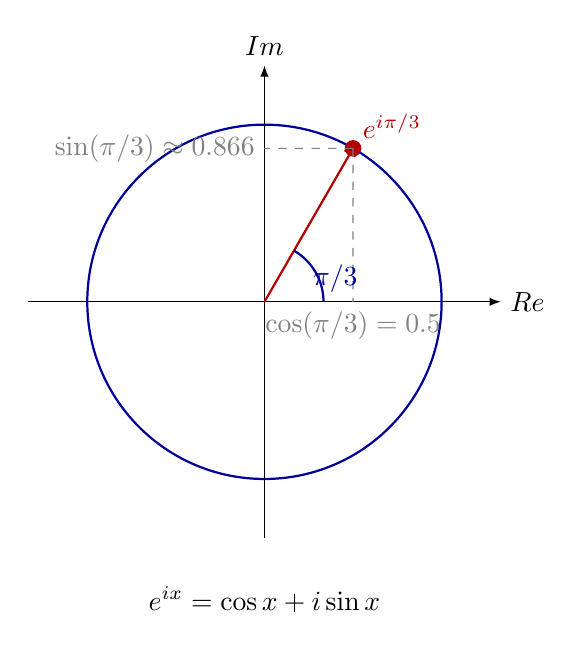
\begin{tikzpicture}[scale=1.5]
  \draw[blue!60!black, thick] (0,0) circle (1.5cm);
  \draw[->, >=latex] (-2,0) -- (2,0) node[right] {$\operatorname{Re}$};
  \draw[->, >=latex] (0,-2) -- (0,2) node[above] {$\operatorname{Im}$};
  \coordinate (P) at ({1.5*cos(60)},{1.5*sin(60)});
  \draw[red!70!black, thick, ->] (0,0) -- (P);
  \fill[red!70!black] (P) circle (2pt);
  \draw[dashed, gray] (P) -- ({1.5*cos(60)},0);
  \draw[dashed, gray] (P) -- (0,{1.5*sin(60)});
  \node[red!70!black, above right] at (P) {$e^{i\pi/3}$};
  \node[below, gray] at ({1.5*cos(60)},0) {$\cos(\pi/3) = 0.5$};
  \node[left, gray] at (0,{1.5*sin(60)}) {$\sin(\pi/3) \approx 0.866$};
  \draw[blue!60!black, thick] (0.5,0) arc (0:60:0.5);
  \node[blue!60!black] at (0.6,0.2) {$\pi/3$};
  \node[below=0.5cm] at (0,-2) {$e^{ix} = \cos x + i\sin x$};
\end{tikzpicture}
\caption{Geometric interpretation of Euler's formula on the unit circle}
\label{fig:euler_formula}
\end{figure}

\begin{theorem}[Euler's Formula]
For any real $x$:
\[
e^{ix} = \cos x + i \sin x
\]
\end{theorem}

\begin{proof}
From the Taylor series for $e^z$:
\[
e^{ix} = \sum_{n=0}^\infty \frac{(ix)^n}{n!}
= \sum_{k=0}^\infty \frac{(-1)^k x^{2k}}{(2k)!} + i \sum_{k=0}^\infty \frac{(-1)^k x^{2k+1}}{(2k+1)!}
= \cos x + i \sin x
\]
The even powers of $i$ give $1, -1, 1, -1, \ldots$ producing the cosine series, and the odd
powers give $i, -i, i, -i, \ldots$ producing $i$ times the sine series.
\end{proof}

\subsection{Alternative Proof via Differential Equations}

\begin{theorem}
The function $f(x) = e^{-ix}(\cos x + i\sin x)$ is constant, equal to 1.
\end{theorem}

\begin{proof}
Differentiating:
\[
f'(x) = -ie^{-ix}(\cos x + i\sin x) + e^{-ix}(-\sin x + i\cos x)
= e^{-ix}[-i\cos x + \sin x - \sin x + i\cos x] = 0
\]
Since $f(0) = 1$, we have $f(x) = 1$ for all $x$, giving $e^{ix} = \cos x + i\sin x$.
\end{proof}

\subsection{Proof via Power Series Uniqueness}

\begin{theorem}
The Taylor series for $\cos x + i\sin x$ equals the Taylor series for $e^{ix}$.
\end{theorem}

\begin{proof}
The Taylor series are:
\[
e^{ix} = \sum_{n=0}^\infty \frac{(ix)^n}{n!}, \quad \cos x + i\sin x = \sum_{k=0}^\infty \frac{(-1)^k x^{2k}}{(2k)!} + i\sum_{k=0}^\infty \frac{(-1)^k x^{2k+1}}{(2k+1)!}
\]
Separating even and odd terms in $e^{ix}$:
\[
e^{ix} = \sum_{k=0}^\infty \frac{(ix)^{2k}}{(2k)!} + \sum_{k=0}^\infty \frac{(ix)^{2k+1}}{(2k+1)!}
= \sum_{k=0}^\infty \frac{(-1)^k x^{2k}}{(2k)!} + i\sum_{k=0}^\infty \frac{(-1)^k x^{2k+1}}{(2k+1)!}
\]
which equals $\cos x + i\sin x$.
\end{proof}

\begin{lstlisting}[caption={Euler's formula verification}, label=lst:euler_formula]
from euler import euler_formula, euler_identity
import math

print("Euler's formula: e^(ix) = cos(x) + i sin(x)")
for x in [0, math.pi/6, math.pi/4, math.pi/3, math.pi/2, math.pi]:
    z = euler_formula(x)
    print(f"  x={x:.4f}: e^(ix) = {z.real:.6f} + {z.imag:.6f}i  (cos={math.cos(x):.6f}, sin={math.sin(x):.6f})")

print("Euler's identity: $e^{i\\pi} + 1 = 0$")
result = euler_identity()
print(f"  e^(i\\pi) + 1 = {result.real:.10e} + {result.imag:.10e}i")
\end{lstlisting}

\section{Euler's Identity}

Setting $x = \pi$ gives the famous identity:
\[
e^{i\pi} + 1 = 0
\]

This equation connects five fundamental constants:
\begin{itemize}
    \item $0$ (additive identity)
    \item $1$ (multiplicative identity)
    \item $e$ (base of natural logarithms)
    \item $i$ (imaginary unit)
    \item $\pi$ (circle constant)
\end{itemize}

\begin{example}[Historical Context]
Euler's identity was first stated by Euler in 1748 in his \emph{Introductio in analysin infinitorum}.
The identity unifies:
\begin{itemize}
\item Arithmetic: $0, 1$
\item Algebra: $i$ (solution to $x^2 + 1 = 0$)
\item Analysis: $e$ (base of natural exponential)
\item Geometry: $\pi$ (ratio of circumference to diameter)
\end{itemize}
\end{example}

\section{De Moivre's Formula}

From Euler's formula, De Moivre's formula follows immediately:
\[
(\cos \theta + i \sin \theta)^n = e^{in\theta} = \cos n\theta + i \sin n\theta
\]

\begin{lstlisting}[caption={De Moivre's formula}, label=lst:demoivre]
from euler import de_moivre_formula
import math

print("De Moivre: (cos \theta + i sin \theta)^n = cos n\theta + i sin n\theta")
for n in [2, 3, 4, 5]:
    for theta in [math.pi/6, math.pi/4, math.pi/3]:
        lhs = de_moivre_formula(n, theta)
        rhs = math.cos(n * theta) + 1j * math.sin(n * theta)
        match = abs(lhs - rhs) < 1e-10
        print(f"  n={n}, \theta={theta:.3f}: {lhs.real:.6f}+{lhs.imag:.6f}i  \checkmark={match}")
\end{lstlisting}

\section{Roots of Unity}

The $n$-th roots of unity are solutions to $z^n = 1$:
\[
z_k = e^{2\pi i k / n} = \cos \frac{2\pi k}{n} + i \sin \frac{2\pi k}{n}, \quad k = 0, 1, \ldots, n-1
\]

They form a regular $n$-gon on the unit circle in the complex plane.

\subsection{Properties of Roots of Unity}

\begin{theorem}
The $n$-th roots of unity form a cyclic group under multiplication.
\end{theorem}

\begin{proof}
The product of two roots $e^{2\pi i j/n}$ and $e^{2\pi i k/n}$ is $e^{2\pi i (j+k)/n}$,
which is also an $n$-th root. The identity is $1 = e^{2\pi i \cdot 0/n}$, and the inverse
of $e^{2\pi i k/n}$ is $e^{2\pi i (n-k)/n}$. The group is generated by $e^{2\pi i/n}$.
\end{proof}

\begin{lstlisting}[caption={Roots of unity}, label=lst:roots_unity]
from euler import roots_of_unity
import math

for n in [3, 4, 5, 6, 8]:
    roots = roots_of_unity(n)
    print(f"\n  {n}-th roots of unity:")
    for k, z in enumerate(roots):
        print(f"    k={k}: {z.real:.6f} + {z.imag:.6f}i")
    # Sum should be 0 for n > 1
    total = sum(roots)
    print(f"  Sum = {total.real:.2e} + {total.imag:.2e}i")
\end{lstlisting}

\subsection{Cyclotomic Polynomials}

The $n$-th cyclotomic polynomial $\Phi_n(x)$ is the minimal polynomial whose roots are
the primitive $n$-th roots of unity:
\[
x^n - 1 = \prod_{d|n} \Phi_d(x)
\]

\begin{example}
$\Phi_1(x) = x - 1$, $\Phi_2(x) = x + 1$, $\Phi_3(x) = x^2 + x + 1$, $\Phi_4(x) = x^2 + 1$.
\end{example}

\section{Trigonometric Identities from Euler's Formula}

Euler's formula makes deriving trig identities easy:
\[
\cos(a+b) = \cos a \cos b - \sin a \sin b
\]
\[
\sin(a+b) = \sin a \cos b + \cos a \sin b
\]

\begin{proof}
Using $e^{i(a+b)} = e^{ia} \cdot e^{ib}$:
\[
(\cos a + i\sin a)(\cos b + i\sin b) = (\cos a \cos b - \sin a \sin b) + i(\sin a \cos b + \cos a \sin b)
\]
Equating real and imaginary parts gives the addition formulas.
\end{proof}

\begin{lstlisting}[caption={Deriving trig identities}, label=lst:trig_ids]
from euler import euler_formula
import math

def cos_sum(a, b):
    return math.cos(a+b)

def sin_sum(a, b):
    return math.sin(a+b)

# Using e^(i(a+b)) = e^(ia) e^(ib)
a, b = math.pi/3, math.pi/4
e_ia = euler_formula(a)
e_ib = euler_formula(b)
e_iab = e_ia * e_ib

print(f"cos({a:.3f}+{b:.3f}) = {e_iab.real:.6f} (formula: {math.cos(a)*math.cos(b) - math.sin(a)*math.sin(b):.6f})")
print(f"sin({a:.3f}+{b:.3f}) = {e_iab.imag:.6f} (formula: {math.sin(a)*math.cos(b) + math.cos(a)*math.sin(b):.6f})")
\end{lstlisting}

\section{Geometric Interpretation}

Euler's formula $e^{ix} = \cos x + i \sin x$ represents a rotation in the complex plane.
For real $x$, the point $e^{ix}$ lies on the unit circle at angle $x$ from the positive
real axis. As $x$ increases, the point traces the circle counterclockwise.

\begin{itemize}
\item $e^{i \cdot 0} = 1$ (angle 0)
\item $e^{i \pi/2} = i$ (angle 90$^\circ$)
\item $e^{i \pi} = -1$ (angle 180$^\circ$)
\item $e^{i 3\pi/2} = -i$ (angle 270$^\circ$)
\item $e^{i 2\pi} = 1$ (angle 360$^\circ$)
\end{itemize}

\subsection{Rotation Formula}

Multiplication by $e^{i\theta}$ rotates a complex number by angle $\theta$:
\[
z \cdot e^{i\theta} = |z| e^{i(\arg z + \theta)}
\]

\section{Computational Complexity}

\subsection{Euler's Formula}
Computing $e^{ix}$ directly via complex exponential:
\begin{itemize}
\item Time: $O(1)$ for fixed-precision arithmetic
\item Memory: $O(1)$
\end{itemize}

Computing via Taylor series with $N$ terms:
\begin{itemize}
\item Time: $O(N)$ arithmetic operations
\item Convergence: rapid for $|x| < 1$, slower for larger $x$ (use reduction modulo $2\pi$)
\end{itemize}

\subsection{Roots of Unity}
Computing all $n$-th roots of unity:
\begin{itemize}
\item Time: $O(n \log n)$ using FFT-based methods, or $O(n)$ with direct computation
\item Memory: $O(n)$ to store all roots
\end{itemize}

\section{Applications}

\begin{itemize}
\item \textbf{Signal Processing:} Euler's formula is the foundation of Fourier analysis,
converting between time-domain and frequency-domain representations.
\item \textbf{Electrical Engineering:} Complex exponentials represent AC circuits
using phasors: $V(t) = V_0 e^{i\omega t}$.
\item \textbf{Quantum Mechanics:} Wave functions use $e^{i(kx - \omega t)}$ as solutions
to the Schr\\"oe"dinger equation.
\item \textbf{Computer Graphics:} 2D rotations use complex multiplication: $z' = z \cdot e^{i\theta}$.
\item \textbf{Control Theory:} Laplace transforms use $e^{st}$ for system analysis.
\item \textbf{Probability:} Characteristic functions use $\phi(t) = E[e^{itX}]$.
\end{itemize}

\subsection{Fourier Analysis}

Any periodic function $f(t)$ with period $T$ can be represented as:
\[
f(t) = \sum_{n=-\infty}^{\infty} c_n e^{2\pi i n t / T}
\]
where $c_n = \frac{1}{T}\int_0^T f(t) e^{-2\pi i n t / T} dt$.

\subsection{Phasor Representation in AC Circuits}

For an AC circuit with voltage $V(t) = V_0 \cos(\omega t)$, we represent:
\[
V(t) = \operatorname{Re}(V_0 e^{i\omega t})
\]
This simplifies circuit analysis by converting differential equations to algebraic ones.

\section{Frequently Asked Questions}

\begin{itemize}
\item \textbf{Q: Why is Euler's formula called ``the most beautiful equation''?} \\
Euler's identity $e^{i\pi} + 1 = 0$ connects five fundamental mathematical constants ($0, 1, e, i, \pi$) using three basic operations (addition, multiplication, exponentiation). No other equation unites so many foundational concepts in such a compact form.

\item \textbf{Q: How do I compute $e^{ix}$ in Python?} \\
Use Python's complex numbers: `cmath.exp(1j * x)` or manually as `math.cos(x) + 1j * math.sin(x)`. The built-in `euler_formula(x)` function in our library implements this. Always verify that $|e^{ix}| = 1$ as a sanity check.

\item \textbf{Q: Why does the Taylor series proof of Euler's formula work?} \\
The Taylor series for $e^{ix}$ naturally splits into real and imaginary parts: the even powers give $\cos x$ and the odd powers give $i \sin x$. Since all three series converge absolutely for all $x$, the rearrangement is justified.

\item \textbf{Q: What are the $n$-th roots of unity and why do they form a regular polygon?} \\
The $n$-th roots of unity are $e^{2\pi i k/n}$ for $k = 0, \ldots, n-1$. These lie on the unit circle at equal angular intervals of $2\pi/n$, forming a regular $n$-gon inscribed in the unit circle. Their sum is always 0 for $n > 1$.

\item \textbf{Q: How does De Moivre's formula follow from Euler's formula?} \\
$(\cos \theta + i \sin \theta)^n = (e^{i\theta})^n = e^{in\theta} = \cos(n\theta) + i \sin(n\theta)$. The proof is immediate from the exponential form. De Moivre originally stated this in 1703, before Euler's formula was discovered.

\item \textbf{Q: Can Euler's formula be extended to quaternions?} \\
Yes. For a quaternion $q = a + bi + cj + dk$ with vector part $\mathbf{v} = (b,c,d)$ and $|\mathbf{v}| = \theta$, we have $e^q = e^a (\cos \theta + \frac{\mathbf{v}}{\theta} \sin \theta)$. This generalizes the planar rotation to 3D rotations.

\item \textbf{Q: What is the geometric meaning of $e^{ix}$?} \\
$e^{ix}$ represents a point on the unit circle at angle $x$ from the positive real axis. It can be viewed as a rotation operator: multiplying any complex number by $e^{ix}$ rotates it by angle $x$ about the origin.
\end{itemize}

\section{Exercises}

\begin{exercise}
Prove $\cos 3\theta = 4\cos^3\theta - 3\cos\theta$ using Euler's formula.
\end{exercise}

\begin{exercise}
Find all solutions to $z^5 = -1$ and plot them in the complex plane.
\end{exercise}

\begin{exercise}
Show that $\prod_{k=1}^{n-1} \sin(\pi k/n) = n/2^{n-1}$ using roots of unity.
\end{exercise}

\begin{exercise}[Proof]
Prove De Moivre's formula $(\cos\theta + i\sin\theta)^n = \cos n\theta + i\sin n\theta$ by induction.
\end{exercise}

\begin{exercise}
Use Euler's formula to derive the half-angle formulas: $\cos^2(x/2) = \frac{1+\cos x}{2}$ and $\sin^2(x/2) = \frac{1-\cos x}{2}$.
\end{exercise}

\begin{exercise}[Computational]
Implement a function that plots the $n$-th roots of unity for $n = 3, 4, 5, 6, 8$ on the complex plane.
\end{exercise}

\begin{exercise}
Prove that $\sin x = \frac{e^{ix} - e^{-ix}}{2i}$ and $\cos x = \frac{e^{ix} + e^{-ix}}{2}$ using Euler's formula.
\end{exercise}

\begin{exercise}
Show that $|e^{z}| = e^{\operatorname{Re}(z)}$ for any complex number $z$.
\end{exercise}

\begin{exercise}
Prove the addition formulas for hyperbolic functions: $\cosh(x+y) = \cosh x \cosh y + \sinh x \sinh y$ and $\sinh(x+y) = \sinh x \cosh y + \cosh x \sinh y$.
\end{exercise}
